\documentclass[aps,prab,reprint,superscriptaddress,nofootinbib]{revtex4-2}

\usepackage[T1]{fontenc}
\usepackage[utf8]{inputenc}
\usepackage{graphicx}
\usepackage{amsmath,amssymb}
\usepackage{bm}
\usepackage{booktabs}
\usepackage[colorlinks=true,linkcolor=blue,citecolor=blue,urlcolor=blue]{hyperref}
\usepackage{orcidlink}
\usepackage{xcolor}

% Two versions from one source: \def\showtodos{} before \input → TODO notes visible.
\newif\iftodo
\ifdefined\showtodos\todotrue\fi
\newcommand{\todo}[1]{\iftodo{\color{red}\textbf{TODO:} #1}\fi}

\begin{document}

\title{Accessing the symmetric component of quadrupole misalignment through
counter-rotating closed orbits in EDM storage rings}

\author{I. Abedrabbo}
\affiliation{Istinye University, Istanbul, T\"urkiye}
\author{S. Hac{\i}\"omero\u{g}lu\,\orcidlink{0000-0002-8207-4219}}
\email{selcuk.haciomeroglu@istinye.edu.tr}
\affiliation{Istinye University, Istanbul, T\"urkiye}

\begin{abstract}
In the storage ring proposed to measure the proton electric dipole moment (EDM), micron-level
quadrupole misalignments mimic a genuine EDM through a geometric (Berry) phase; at $10~\mu$m rms the
false signal exceeds the target sensitivity of $10^{-29}~e\cdot$cm by one to three orders of magnitude.
Decomposing the misalignment of each focusing--defocusing pair into an antisymmetric and a symmetric
component, we show that the symmetric component produces a closed-orbit distortion four to seven times
weaker than the antisymmetric one at low harmonics, so that single-beam orbit correction leaves it largely
in place. Using symplectic beam and spin tracking with the false EDM evaluated at the frozen-spin energy, we
show that a joint fit of the two counter-rotating closed orbits recovers the symmetric component: the
antisymmetric component appears in the difference of the two orbits, the symmetric one in their sum.
Because static monitor offsets are degenerate with the symmetric component in the sum, the scheme is a
drift monitor operating relative to a beam-based-alignment reference. We quantify its domain of validity
against the errors that compete in the same channel: monitor motion, electrostatic deflector drift,
corrector type, correlated (ground-motion-like) misalignment, and a one-week operating scenario. With
quadrupole-mounted dipole correctors, deflector field trims, and monitors either fixed or rigidly attached
to the quadrupoles and modeled accordingly, two-beam monitoring keeps the false EDM well below target
between beam-based alignments without quadrupole polarity reversal.
\end{abstract}
\maketitle

%======================================================================
\section{INTRODUCTION}
\label{sec:intro}
%======================================================================
\subsection{Frozen spin method and the false EDM}
\label{sec:frozenspin}
A permanent electric dipole moment of an elementary particle violates both parity (P) and time-reversal (T)
symmetries and, assuming CPT invariance, implies CP violation. The Standard Model predicts about
$10^{-31}~e\cdot$cm for the proton EDM, so any observation above this level indicates physics beyond the
Standard Model. The proposed storage-ring proton EDM experiment~\cite{srEDM,omarov} uses the frozen-spin
method: protons are stored at the ``magic'' momentum ($p\approx0.7$~GeV/$c$), at which the spin follows the
momentum in the horizontal plane. The EDM then couples to the radial electric field of the deflectors and
precesses the spin out of the plane, which is measured by polarimetry~\cite{polarimeter}, at the rate
\begin{equation}
f \equiv \frac{dS_y}{dt}, \qquad d=10^{-29}~e\cdot\text{cm} \longleftrightarrow f \approx 1~\text{nrad/s}.
\end{equation}
Couplings of the magnetic dipole moment that mimic this precession constitute false EDM signals. This paper
studies the false EDM caused by misaligned magnetic quadrupoles.

The magnetic field at the center of a quadrupole is zero. A misaligned quadrupole exposes the beam to a
dipole field proportional to the misalignment: a vertical misalignment $dy$ gives a radial field that
precesses the spin in the vertical plane, a horizontal misalignment $dx$ a vertical field that precesses it
in the horizontal plane. Each precession alone averages out along the closed orbit, but rotations about
orthogonal axes do not commute, and the sequence leaves a net out-of-plane rotation per turn. This geometric
(Berry) phase~\cite{berry1984,aharonov1987,farley2004,haciomeroglu2019} makes the false EDM bilinear in the
horizontal and vertical misalignments,
\begin{equation}
f_\text{false} \propto dx\cdot dy \quad \rightarrow \quad \vert f_\text{false} \vert \propto \sigma^2,
\label{Eq:sigma_quadratic}
\end{equation}
where $\sigma$ is the rms misalignment. At $\sigma=10~\mu$m the false signal is $10$--$10^3$ times the
target, depending on the misalignment pattern (Sec.~\ref{sec:benchmark}).

\subsection{Ring design}
\label{sec:ring}
We use the symmetric-hybrid ring of Ref.~\cite{omarov}: 24 FODO cells of electrostatic deflectors and
magnetic quadrupoles. The focusing (QF) and defocusing (QD) quadrupoles have the same gradient magnitude
($g=0.2$~T/m), separated by drifts and deflectors,
QF $\rightarrow$ drift $\rightarrow$ deflector $\rightarrow$ drift $\rightarrow$ QD $\rightarrow$ drift
$\rightarrow$ deflector $\rightarrow$ drift. The deflectors are cylindrical capacitors of 95.5~m radius
with $E_0=4.4$~MV/m. Figure~\ref{fig:optics} shows the cell layout and the beta functions, and
Table~\ref{tbl:ring_parameters} lists the main parameters.

\begin{figure}[tb]
\centering
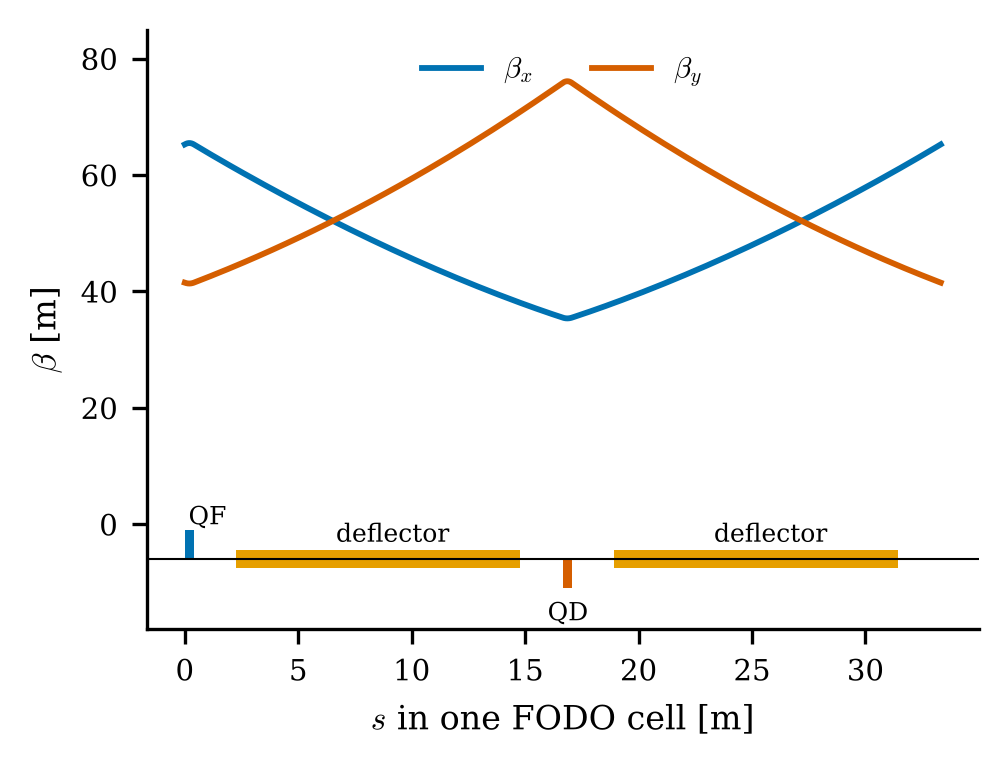
\includegraphics[width=\linewidth]{fig_v2_optics.png}
\caption{One FODO cell of the ring: element layout (bottom) and beta functions. The vertical focusing of
the deflectors is zero ($n=1$); their horizontal focusing is included through the measured horizontal
tune. The cell is repeated 24 times.}
\label{fig:optics}
\end{figure}

\begin{table}[tb]
\centering
\caption{Ring and beam parameters, consistent with Ref.~\cite{omarov}.}
\begin{tabular}{ll}
\hline
Parameter & Value \\
\hline
Number of FODO cells & 24 \\
Ring radius / circumference & 95.5 m / 800 m \\
Beam momentum & 0.7007 GeV/$c$ \\
Relativistic $\beta$, $\gamma$ & 0.598, 1.248 \\
Revolution time & 4.46 $\mu$s \\
Betatron tunes ($Q_x, Q_y$) & (2.64, 2.3) \\
$\beta$ at QF / QD, horizontal & 65 m / 35 m \\
$\beta$ at QF / QD, vertical & 42 m / 76 m \\
Dispersion ($D^\text{max}$) & 34 m \\
Slip factor & $-0.25$ \\
\hline
\end{tabular}
\label{tbl:ring_parameters}
\end{table}

\subsection{Symmetric and antisymmetric components}
\label{sec:symanti}
The quadrupoles are indexed $n=0,\dots,47$; cell $k=0,\dots,23$ contains QF $n=2k$ and QD $n=2k+1$. Let
$v[n]$ be the misalignment of quadrupole $n$ in one plane. Within each cell we define
\begin{equation}
\begin{split}
v^s[2k] &= v^s[2k+1] = \tfrac{1}{2}\left(v[2k] + v[2k+1]\right), \\
v^a[2k] &= -v^a[2k+1] = \tfrac{1}{2}\left(v[2k] - v[2k+1]\right),
\end{split}
\label{Eq:symanti}
\end{equation}
so that $v[n]=v^s[n]+v^a[n]$ for every $n$. The symmetric component $v^s$ displaces QF and QD of a cell
in the same direction, the antisymmetric component $v^a$ in opposite directions. The projections
$P_s$ and $P_a=I-P_s$ defined by Eq.~\eqref{Eq:symanti} are orthogonal, and each component spans a
24-dimensional subspace. The same decomposition is applied to the horizontal ($v_x$) and vertical ($v_y$)
misalignments.

\subsection{Correction of quadrupole misalignment and contribution of this work}
\label{sec:correction}
Reference~\cite{omarov} corrects the misalignment in two steps. Beam-based alignment (BBA) varies the
gradient of each quadrupole and steers the beam until it no longer responds, i.e., through the magnetic
center; it can be accelerated by ac excitation~\cite{marti} and parallelized~\cite{huang}. The residual is
then cancelled by combining four configurations: clockwise (CW) and counterclockwise (CCW) beams, each at
both quadrupole polarities ($g\rightarrow-g$) (Eq.~(C2) of Ref.~\cite{omarov}). This is powerful but costs
running time and requires a lattice symmetric between the two polarities.

Standard orbit correction (OC), based on the singular value decomposition (SVD) of the orbit response
matrix~\cite{chung1993,ziemann,mirza,wegscheider}, runs continuously and noninvasively. We show that a
single-beam OC leaves most of the symmetric component in place, because that component distorts the
closed orbit weakly (Sec.~\ref{sec:mechanism}), whereas a joint fit of the two counter-rotating (CR) beams
recovers it (Sec.~\ref{sec:croc}). Static monitor offsets are degenerate with the symmetric component in
the two-beam fit, so the scheme is a drift monitor relative to a BBA reference. Section~\ref{sec:validity}
quantifies where the scheme works, against the error sources raised in its review: monitor motion,
deflector errors, corrector type and correlated misalignment; Sec.~\ref{sec:time} follows it through a
one-week operating scenario.

%======================================================================
\section{SIMULATION METHOD}
\label{sec:simulation}
%======================================================================
\subsection{Beam and spin tracking}
\label{sec:tracking}
All results were obtained with an in-house code that tracks one particle and its spin through the lattice
of Sec.~\ref{sec:ring} with a Gauss--Legendre symplectic integrator~\cite{hairer}, the spin following the
Thomas--BMT equation~\cite{bmt1959}. The deflector field is $E_r=E_0R_0/R$ inside the deflector and zero
outside (hard edge). Quadrupole misalignments, rolls and gradient errors, deflector field errors and rolls,
and dipole correctors are ring parameters. With the EDM coupling set to $d_p=10^{-29}~e\cdot$cm the code
gives $dS_y/dt=9.8\times10^{-10}$~rad/s with opposite signs for the two beam directions, as expected; all
false-EDM results are obtained with the EDM coupling switched off.

\subsection{Response matrices}
\label{sec:respmodel}
The orbit response matrices $R$ (BPM reading per unit quadrupole misalignment, $48\times48$ per plane and
per beam direction) were obtained by tracking. Since the quadrupole kick reverses with the beam direction,
$R_\text{CW}\approx-R_\text{CCW}$; the mean column correlation is $-0.95$ in both planes, the deviation
coming from the electric bending that does not reverse. The analytical expression
\begin{equation}
R_{ij} =  (KL)_j \frac{\sqrt{\beta_i \beta_j}}{2 \sin \pi Q}\cos(\vert \Delta \psi_{ij} \vert - \pi Q)
\label{Eq:response_matrix}
\end{equation}
agrees with the tracked matrices within a few percent vertically, but not horizontally, where the
deflector focusing matters; tracked matrices are used throughout.

\subsection{False EDM estimation at the frozen-spin energy}
\label{sec:estimator}
A particle launched off the closed orbit performs betatron oscillations whose effect on $S_y$ is orders of
magnitude larger than the false EDM. We therefore (i) find the four-dimensional closed orbit
$(x,x',y,y')$ by minimizing the turn-by-turn position variance, (ii) launch the particle on it with the
spin longitudinal, and (iii) fit
\begin{equation*}
S_y(t) = a + bt + \sum_k [c_k \cos \omega_k t + d_k \sin \omega_k t],
\end{equation*}
keeping the secular slope $b$.

The closed orbit fixes the launch position and angle but not the energy, and the false EDM is very
sensitive to it: around $\sigma=10~\mu$m, a relative momentum change $\delta=10^{-7}$ changes $f$ by about
$290\times$ the target, while the horizontal spin precession rate changes by
$d\omega_h/d\delta=-5.24\times10^{6}$~rad/s, independent of the misalignment. In a misaligned lattice the
energy at which the horizontal spin is frozen ($\omega_h=0$) differs from the design magic energy by an
amount proportional to the misalignment (here $\sim10^{-7}$). The experiment keeps $\omega_h=0$ by a
feedback on the measured horizontal spin phase~\cite{jedi_phaselock}, so that is the reference we use: each
false EDM is measured at two energies, $f_0,\omega_0$ and $f_1,\omega_1$ with
$\delta_1=-\omega_0/(d\omega_h/d\delta)$, and interpolated to $\omega_h=0$,
$f^*=f_0+(f_1-f_0)(0-\omega_0)/(\omega_1-\omega_0)$. Both quantities are linear in $\delta$ over
$|\delta|\le10^{-6}$; in practice $|\omega_1|\lesssim3\times10^{-4}$~rad/s, so the second point lies at the
frozen-spin energy. A beam with a symmetric momentum spread around this energy gives the same mean signal,
since $f$ is linear in $\delta$.

A launch at fixed momentum $|p|=p_\text{magic}$ instead makes the result depend on the launch point: with
hard-edge deflectors the momentum along a distorted closed orbit varies from cell to cell by
$\sim10^{-7}$, so each launch point selects a different energy. Moving the launch point of the same
misalignment pattern by 6, 12 and 18 cells changes the fixed-momentum result from $1088$ to $2729$, $-456$
and $95$ times the target, while the frozen-spin result stays at $82.04$, $81.90$, $81.89$ and $81.94$.
The four frozen-spin solutions are the same orbit: their cell-to-cell momentum differences agree to four
digits with those measured directly along one closed orbit. The difference between the two procedures
grows with the closed-orbit amplitude at launch, so it is negligible for well-corrected orbits but not for
uncorrected ones (Appendix~\ref{app:launch}).
\todo{Cite our earlier arXiv paper where the frozen-spin energy shift with lattice imperfections is discussed.}

\subsection{Benchmarks}
\label{sec:benchmark}
With perfectly aligned quadrupoles the estimator returns zero within the numerical floor
($\approx0.008\times$target with the settings used for the scans, $<0.003$ with the full settings).
Switching on the EDM gives the expected rate above. A uniform roll $\phi$ of all deflectors produces a
first-order false EDM $|f|=G\gamma\cdot2\pi\phi/T_\text{rev}$ (Sec.~\ref{sec:defl}), reproduced to $10^{-5}$
relative accuracy and with the same sign for both beam directions. Restoring random quadrupole
misalignments, the false EDM scales as $\sigma^p$ with $p=2.0002$ over $\sigma=2.5$--$10~\mu$m (three
patterns), confirming the geometric phase. Note that this test does not validate the absolute value: a
measurement at a wrong energy carries an error that also scales as $\sigma^2$, because both the energy
offset and $df/d\delta$ are proportional to $\sigma$.

%======================================================================
\section{FALSE EDM MECHANISM}
\label{sec:mechanism}
%======================================================================
\subsection{Orbit visibility of the two components}
\label{sec:visibility}
A misaligned quadrupole kicks the beam by $\theta\propto g\,v$. Since QF and QD have opposite gradients, an
antisymmetric pattern kicks the beam in the same direction at both quadrupoles of a cell, a symmetric
pattern in opposite directions. In the smooth-focusing picture the symmetric pattern is therefore a pure
cell harmonic $k=24$ and its orbit response, $G_k\propto1/|Q^2-k^2|$, would be about 100 times weaker than
that of low harmonics. The measured response is very different [Fig.~\ref{fig:modes}(a)]: for a
misalignment pattern of cell harmonic $m$, the symmetric-to-antisymmetric orbit gain ratio is
$0.15$--$0.25$ for $m\le3$ and rises to unity at $m=12$. The reason is that the orbit response to a kick is
weighted by $\sqrt{\beta}$, which differs strongly between QF and QD (Table~\ref{tbl:ring_parameters}).
The two kicks of a symmetric cell pattern therefore do not cancel; the net kick, relative to that of an
antisymmetric pattern, is $|\sqrt{\beta_F}-\sqrt{\beta_D}|/(\sqrt{\beta_F}+\sqrt{\beta_D})\approx0.15$ in
both planes, in agreement with the measured low-harmonic ratio. The symmetric component is thus not
invisible to the orbit, but four to seven times weaker than the antisymmetric one at the low harmonics
where both the orbit and, as shown below, the spin are most sensitive.

The same structure appears in the SVD of $R$ [Fig.~\ref{fig:modes}(b)]: ordering the singular values, the
right singular vectors of the smallest ones are predominantly symmetric. A truncated SVD with a threshold of
$10^{-2}$ removes 17 (horizontal) and 24 (vertical) of the 48 directions of a single-beam matrix,
mostly symmetric ones.

\begin{figure*}[tb]
\centering
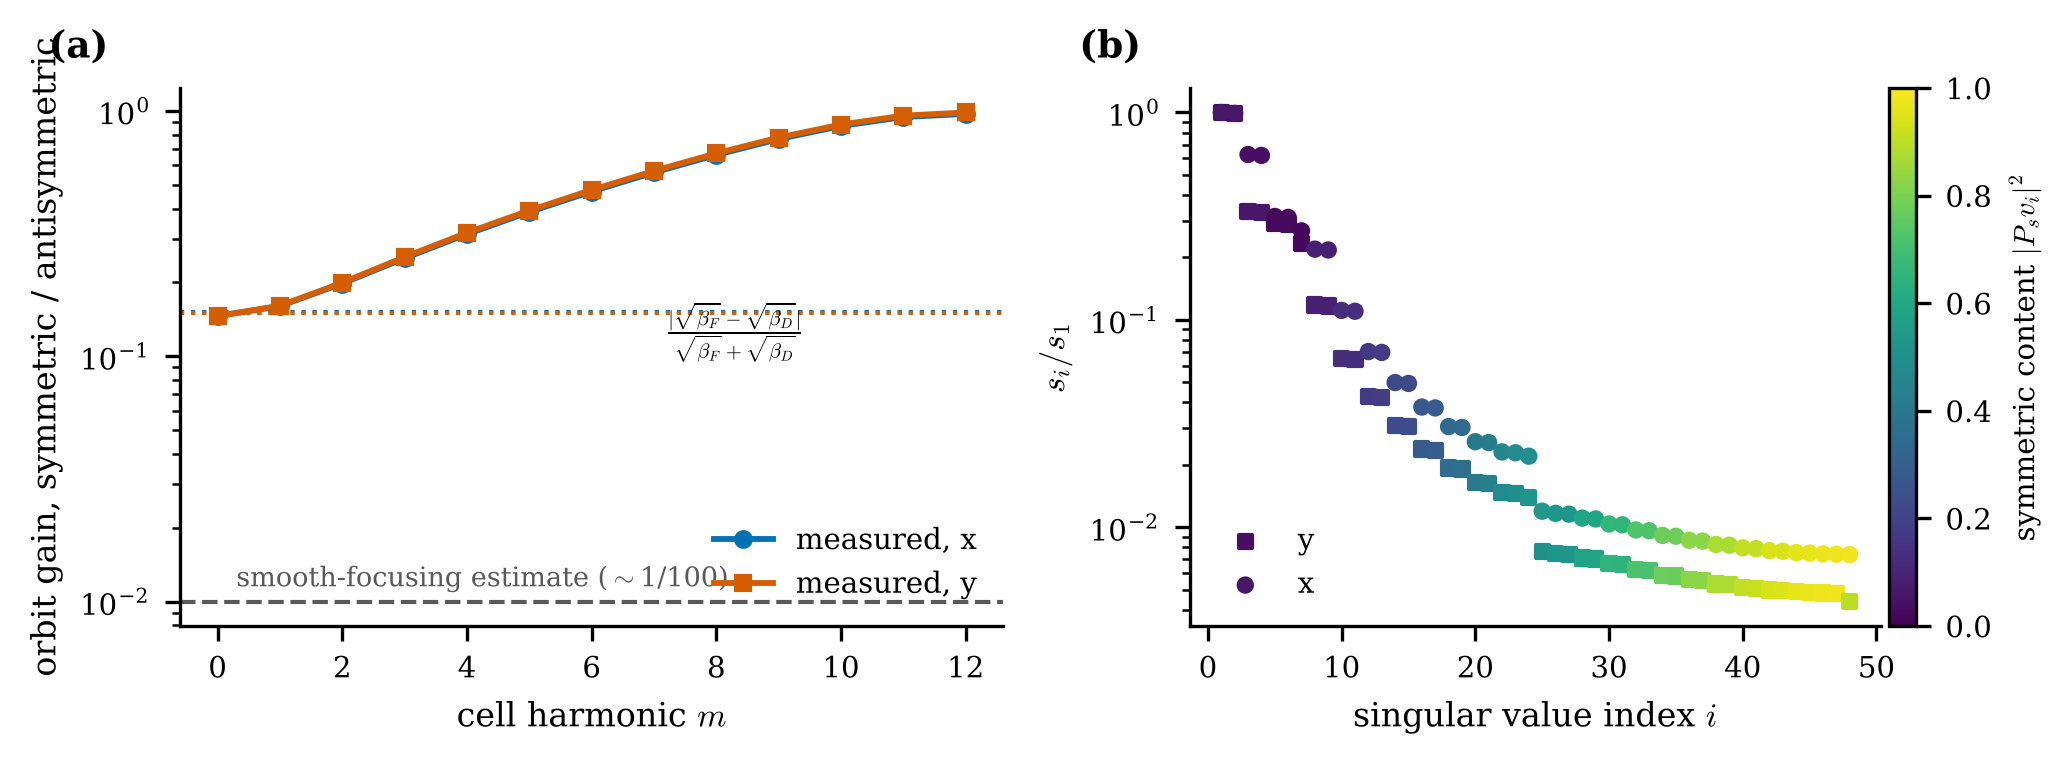
\includegraphics[width=\linewidth]{fig_v2_modes.png}
\caption{Orbit visibility of the two components. (a) Ratio of the closed-orbit gain of a symmetric to an
antisymmetric misalignment pattern of cell harmonic $m$ (tracked response matrices, CCW beam). Dotted:
$\sqrt{\beta}$ estimate; dashed: smooth-focusing estimate. (b) Normalized singular values of the
single-beam response matrix, colored by the symmetric content of the corresponding right singular vector.}
\label{fig:modes}
\end{figure*}

\subsection{False EDM as a bilinear functional}
\label{sec:bilinear}
Equation~\eqref{Eq:sigma_quadratic} generalizes to $f=\sum_{ij}W_{ij}v_{x,i}v_{y,j}=F(v_x,v_y)$, with a
lattice-defined kernel $W$. Splitting both patterns,
\begin{equation}
f= F(v_x^s, v_y^s) + F(v_x^s, v_y^a) + F(v_x^a, v_y^s) + F(v_x^a, v_y^a).
\end{equation}
\IfFileExists{fig_v2_channels.png}{Figure~\ref{Fig:channels} shows the four channels measured
separately; they add up to the full signal and each scales as $\sigma^2$.}{}
The antisymmetric content dominates the false EDM as it dominates the orbit, but by a smaller factor:
relative to its orbit visibility, the symmetric component is the more harmful one. Correcting the orbit with a single beam therefore reduces $\sigma$ but does not
guarantee the suppression of the geometric phase.
\todo{Figure~2 (channels) to be regenerated with the frozen-spin estimator (run in progress:
revizyon/makale\_yeniden\_olcum.py, kind \texttt{ch}); the old figure used fixed-momentum launch.}

\IfFileExists{fig_v2_channels.png}{%
\begin{figure*}[tb]
\includegraphics[width=\linewidth]{fig_v2_channels.png}
\caption{Four channels of the false EDM, measured separately at the frozen-spin energy (CCW beam). (a)
$\sigma=10~\mu$m, three patterns; (b) $\sigma^2$ scaling of each channel, one pattern.}
\label{Fig:channels}
\end{figure*}}{}

%======================================================================
\section{CORRECTION SCHEMES}
\label{sec:schemes}
%======================================================================
\subsection{Beam-based alignment}
\label{sec:bba}
BBA aligns the quadrupoles one at a time and does not invert the global response matrix, so it treats the
two components alike. With $\approx1\%$ random gradient errors, varying one quadrupole gradient changes the
optics of the whole ring (``breathing'', Appendix~\ref{app:breathing}) and biases the null by an amount
proportional to the closed-orbit distortion; iterating removes the bias. In our simulation eight passes
reduced the rms symmetric misalignment from 4.3 (3.3)~$\mu$m to 0.9 (0.06)~$\mu$m horizontally
(vertically), bringing the false EDM below the target.
\todo{The BBA false-EDM values were obtained with the fixed-momentum launch and their residual patterns
were not stored; re-run classic\_bba\_iter.py with the frozen-spin estimator (about 19 h, office machine).
At pass 8 the closed orbit is small, so the launch bias is expected to be small (App.~A).}

\subsection{Single-beam orbit correction}
\label{sec:oc1}
Standard OC estimates the misalignment as $\hat v=R^{+}y$ with a truncated-SVD pseudo-inverse and cancels
it. Its limitation for the symmetric component is conditioning: the symmetric directions have the smallest
singular values (Fig.~\ref{fig:modes}) and are the first removed by the truncation. The result therefore
depends strongly on the threshold. With the threshold set to $10^{-2}$ of the largest singular value, a
5~$\mu$m symmetric drift is reduced only to $3.9~\mu$m; with $3\times10^{-3}$ it is reduced to
$0.05~\mu$m (14~nm BPM noise). The threshold need not be chosen with knowledge of the true misalignment: the
discrepancy principle---the largest threshold for which the fit residual $\|S\hat v-y\|$ reaches the
noise level---reproduces the best threshold within a factor of 1.7 in residual for every estimator used
here, and fails to reach the noise level when the measurement model is wrong, which flags model errors.
We use it throughout. The orbit-difference alternative, which removes BPM offsets by modulating the
quadrupole gradients, suffers from an ill-conditioned difference matrix and from breathing
(Appendices~\ref{app:breathing} and \ref{app:orb_diff_inv}).

\subsection{Two-beam orbit correction}
\label{sec:croc}
The two counter-rotating beams are stored together and read by the same BPMs, separated by bunch timing.
Since the quadrupole kick reverses with the beam direction, the antisymmetric part of the closed orbit
is nearly opposite for the two beams and the symmetric part nearly the same, up to a phase shift from the
reversed order of the two quadrupoles of a cell [Fig.~\ref{fig:orbit_cw_ccw}]. In terms of the sum and
difference of the two response matrices (Frobenius norms, vertical plane), the antisymmetric component
drives the difference channel ($\tfrac12\|(R_\text{CW}-R_\text{CCW})P_a\|=45$) and only weakly the sum
($6.8$); the symmetric component appears in both ($6.9$ and $6.5$). In the sum channel the two
components are therefore of equal visibility, while in a single beam the symmetric one is buried under an
antisymmetric response seven times larger. Appendix~\ref{app:sum} gives a two-dimensional illustration.

\begin{figure*}[tb]
\centering
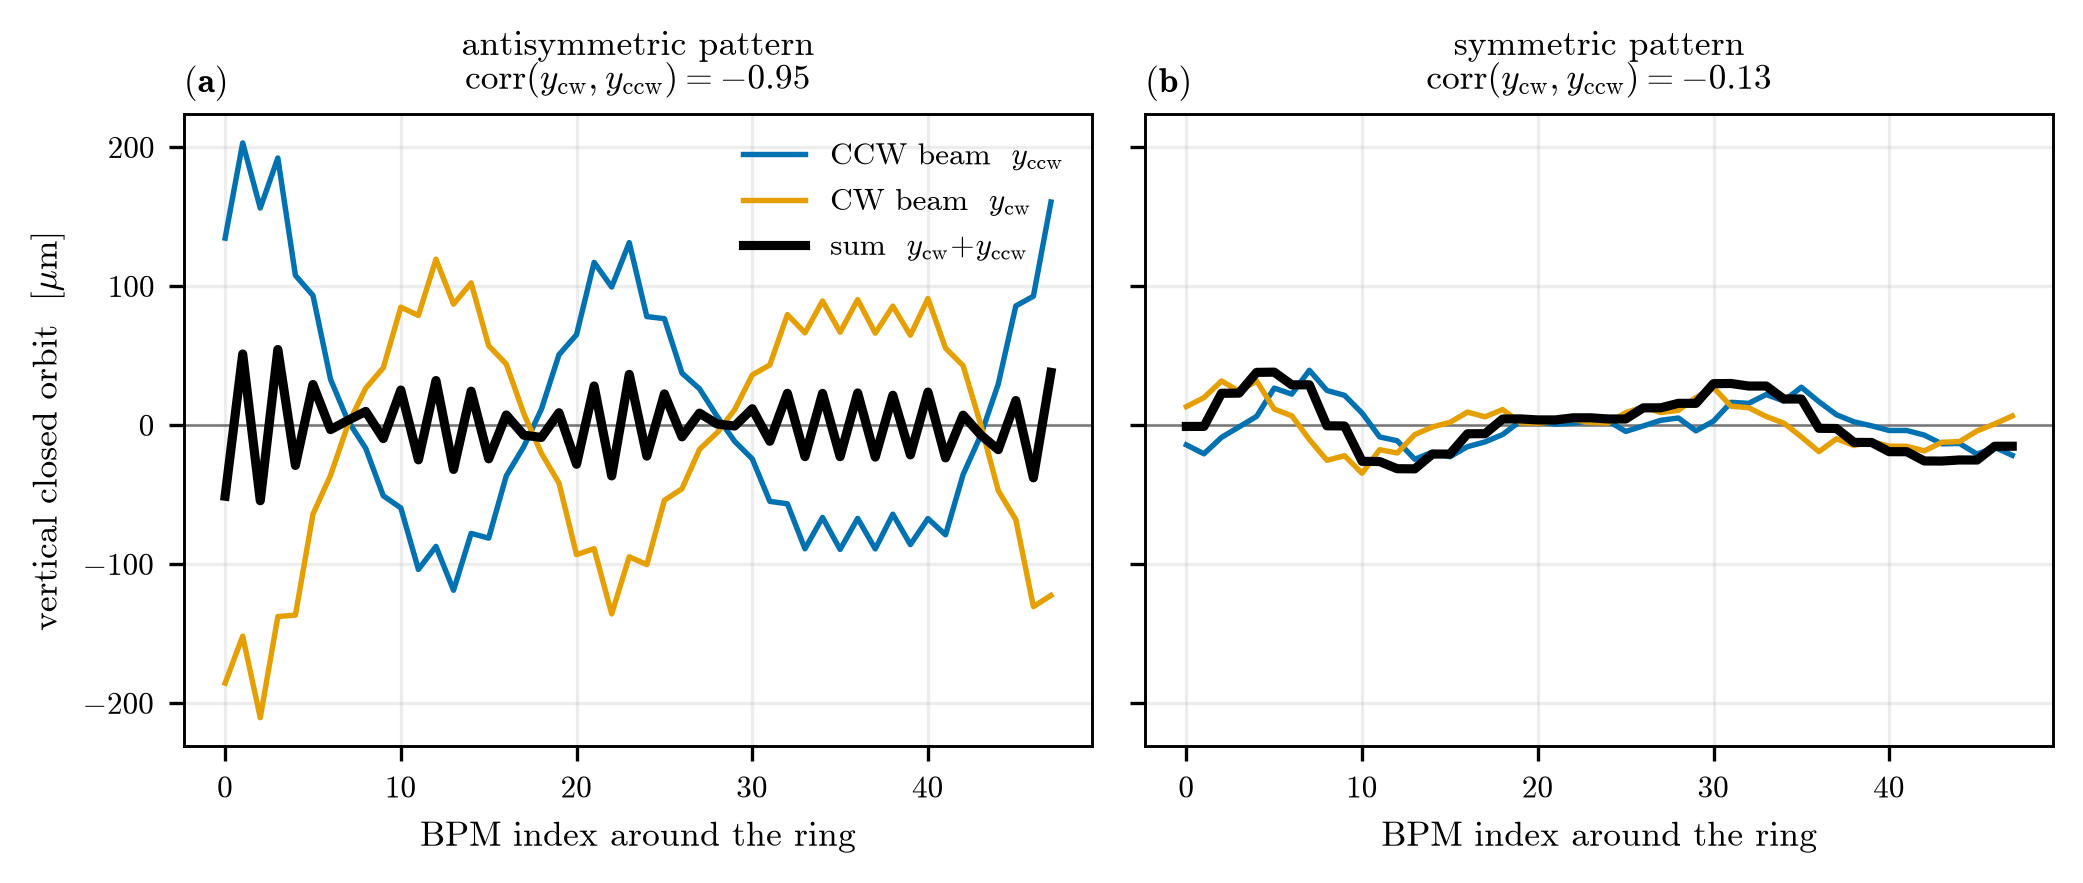
\includegraphics[width=1\linewidth]{fig_orbit_cwccw.png}
\caption{Vertical closed orbits of the two beams for a 10~$\mu$m rms misalignment. (a) Antisymmetric
pattern: the orbits are nearly opposite and their sum (black) is a small residual. (b) Symmetric pattern:
the orbits are nearly equal up to a phase shift and their sum survives.}
\label{fig:orbit_cw_ccw}
\end{figure*}

\paragraph*{Algorithm.} The scheme operates relative to a BBA reference:
\begin{enumerate}
\item After BBA, record the readings of both beams, $y^\text{ref}_\text{CW}$, $y^\text{ref}_\text{CCW}$, and
the corrector settings $c^\text{ref}$.
\item At each step, average the readings of both beams over $T_\text{avg}$ and form the changes
$\Delta y_b=y_b-y^\text{ref}_b$ ($b=$~CW, CCW), adding back the known orbit change from the correctors.
\item Estimate the misalignment drift by the two-beam least-squares fit
\begin{equation}
\Delta\hat v = S^{+}\begin{pmatrix}\Delta y_\text{CW}\\ \Delta y_\text{CCW}\end{pmatrix},\qquad
S=\begin{pmatrix}R_\text{CW}-\rho I\\ R_\text{CCW}-\rho I\end{pmatrix},
\label{eq:twobeamfit}
\end{equation}
with the truncation chosen by the discrepancy principle; $\rho$ describes the monitor mounting
(Sec.~\ref{sec:bpm}; $\rho=0$ for monitors fixed in the laboratory frame).
\item Apply $\Delta\hat v$ with dipole correctors mounted in the quadrupoles (Sec.~\ref{sec:correctors}).
\item Follow the estimated symmetric drift; repeat BBA when its expected accumulation reaches a
predefined threshold.
\end{enumerate}
Static BPM offsets enter both beams identically, i.e. entirely in the sum channel, and are degenerate with
the symmetric misalignment. Without a reference, a 100~$\mu$m rms offset leads to a false EDM about 200
times the target. In the differences of step~2 the static offset cancels; what remains is the change of
the BPM offset relative to the quadrupole center since the last BBA, which we call $\delta$
(Sec.~\ref{sec:bpm}).

\paragraph*{Performance.} Figure~\ref{fig:suppression} compares the schemes for $\sigma=10~\mu$m random
misalignments, 14~nm BPM noise and a fixed threshold of $10^{-2}$, with the false EDM given by the
observable $C=\tfrac12|f_\text{CW}-f_\text{CCW}|$ (the genuine EDM reverses with the beam direction). The
uncorrected machine gives a median of $49\times$ target; single-beam correction $12\times$; two-beam
correction $0.0015\times$, at the numerical floor. The single-beam result improves to the floor with a
lower threshold (Sec.~\ref{sec:oc1}, Table~\ref{tbl:bpm}), so the advantage of the two-beam fit at fixed
threshold mostly reflects conditioning; its decisive advantages appear when the monitors move
(Sec.~\ref{sec:bpm}).
\todo{Fig.~\ref{fig:suppression}: add the 15-seed two-beam point with 0.2\% gradient error (kind tb20)
and the single-beam points at $\sigma=5,20~\mu$m once the re-run finishes.}

\begin{figure}[tb]
\centering
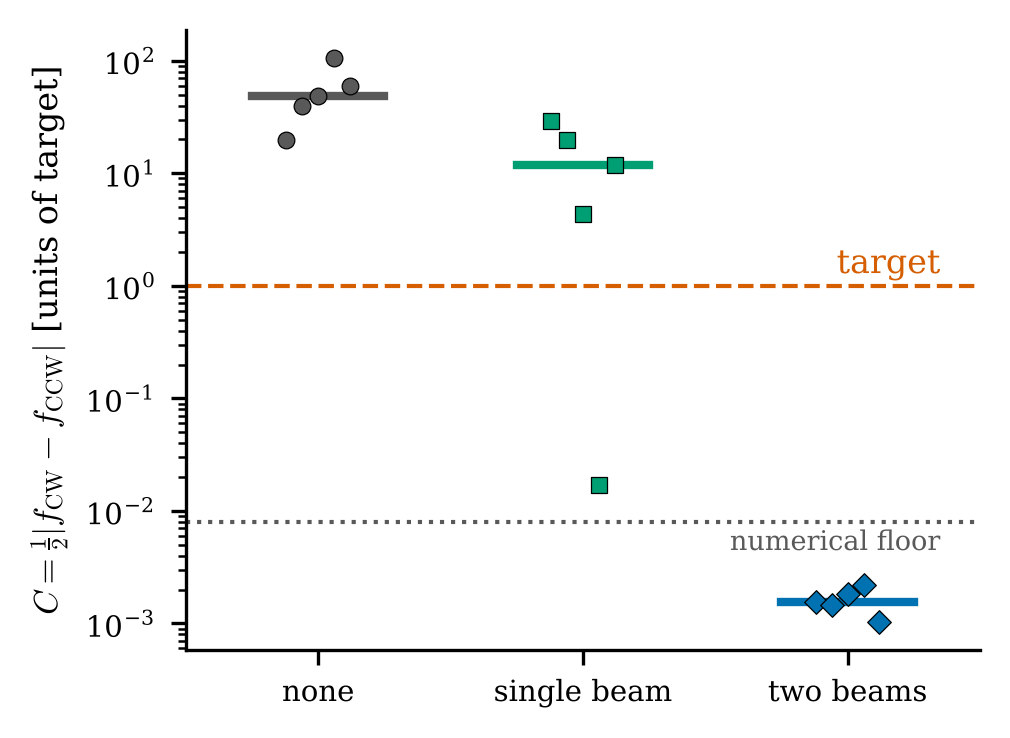
\includegraphics[width=\linewidth]{fig_v2_suppression.png}
\caption{False EDM at $\sigma=10~\mu$m (five patterns, bars = median) without correction, after
single-beam correction and after two-beam correction (14~nm BPM noise, truncation $10^{-2}$, monitors
fixed). Dotted: numerical floor.}
\label{fig:suppression}
\end{figure}

An important practical advantage is that the two-beam correction does not require the quadrupole polarity
reversal of the reference scheme, which needs a second storage per measurement.

%======================================================================
\section{DOMAIN OF VALIDITY}
\label{sec:validity}
%======================================================================
The two-beam fit reads the symmetric component in the sum channel. Any other error that appears in the
same channel competes with it. This section examines those errors. Unless stated otherwise the scenario is
a 5~$\mu$m rms purely symmetric drift after BBA (the component the scheme must catch), 14~nm BPM noise,
and 10 patterns; false EDM values are $C$ in units of the target.

\subsection{Monitor model}
\label{sec:bpm}
A BPM measures the beam relative to its own electrical center. We write the change of the reading of
beam $b$ after BBA as
\begin{equation}
\Delta r_b = R_b\,\Delta v - u + n_b,\qquad u=\rho\,\Delta v+\delta,
\label{eq:bpmmodel}
\end{equation}
where $\rho=0$ describes a monitor fixed in the laboratory frame, $\rho=1$ a monitor rigidly attached to
its quadrupole, and $\delta$ the relative drift between the BPM electrical center and the quadrupole
magnetic center (mechanical and electronic). Long-wavelength ground motion moves quadrupoles and nearby
monitors together, i.e. towards $\rho=1$~\cite{rossbach}. For a rigidly attached monitor the reading is the
beam position relative to the quadrupole center, which is exactly the quantity that drives the false EDM;
even a single beam then sees the symmetric component, through the $-\Delta v$ term.

We compare four estimators: single beam assuming fixed monitors (E1), single beam with $(R-\rho I)$ (E2),
two beams assuming fixed monitors (E3), and two beams with $(R-\rho I)$ (E4, Eq.~\eqref{eq:twobeamfit}).
Table~\ref{tbl:bpm} and Fig.~\ref{fig:bpm}(a) summarize the results.

\begin{table}[tb]
\centering
\caption{Residual symmetric misalignment (200 patterns, median) and false EDM (10 patterns, median and
maximum) for a 5~$\mu$m symmetric drift. Without correction $C=6.3$ (9 of 10 patterns above target).}
\begin{tabular}{llccc}
\hline
$\rho$ & estimator & residual [$\mu$m] & $C$ median & $C$ max \\
\hline
0 & E1 (single beam) & 0.051 & 0.008 & 0.035 \\
0 & E3 (two beams) & 0.017 & 0.005 & 0.012 \\
1 & E1 & 4.88 & 3.5 & 19 \\
1 & E2 & 0.115 & 0.006 & 0.017 \\
1 & E3 & 4.39 & 0.19 & 0.33 \\
1 & E4 & 0.012 & 0.003 & 0.011 \\
\hline
\end{tabular}
\label{tbl:bpm}
\end{table}

Three results stand out. First, with fixed monitors both single- and two-beam fits reach the floor; the
two-beam advantage in the residual is a factor of three, which shrinks to 1.2 for a 0.2\% rms gradient error
in the machine not included in the model. Second, if the monitors follow the quadrupoles but the estimator
assumes fixed monitors (E3), most of the symmetric drift survives (4.4~$\mu$m), yet $C$ stays below target
(0.19, maximum 0.33): the surviving part lies at harmonics far from the betatron tune, to which the spin is
weakly sensitive, while the fit removes 76--78\% of the power at $m=2$--3. The margin, however, is only a
factor of three to five. At $\rho=0.5$ the same estimator gives $C=0.013$. Third, an estimator that knows
the mounting (E2, E4) reaches the floor; E4 tolerates a 10\% error in $\rho$ without leaving the floor,
whereas E2 exceeds the target for one of six patterns at $\hat\rho=0.9$.

\paragraph*{Rigidly attached monitors.} The remaining error is the relative drift $\delta$. With
$\delta$ independent from monitor to monitor [Fig.~\ref{fig:bpm}(b)], the two-beam false EDM stays at the
numerical floor up to $\sigma_\delta=1~\mu$m, while the single-beam one grows as $\sigma_\delta^2$ and
exceeds the target in 7 of 8 patterns at $1~\mu$m. The reconstruction error of the two-beam fit grows as
$1.1\,\sigma_\delta$, but 93\% of its power is in a uniform translation and a tilt of the ring ($m=0,1$):
these are near-null directions of $(R-I)$, because the closed orbit follows a rigid displacement of the
lattice, and for the same reason the spin is insensitive to them---the beam still passes through the
quadrupole centers. Mounting BPMs in or on the quadrupole is standard practice in linacs (TTF2/European
XFEL, CLIC)~\cite{ttf2,pacman}; light sources separate them because of synchrotron-radiation heating of the
girders, which does not apply here. Monitor electronics drifts of 0.1~$\mu$m/h~\cite{sls2} and
$\le1~\mu$m over a week~\cite{aps_mba} are specified in modern light sources, so $\sigma_\delta\lesssim1~\mu$m
between BBA calibrations is consistent with the state of the art.

\begin{figure*}[tb]
\centering
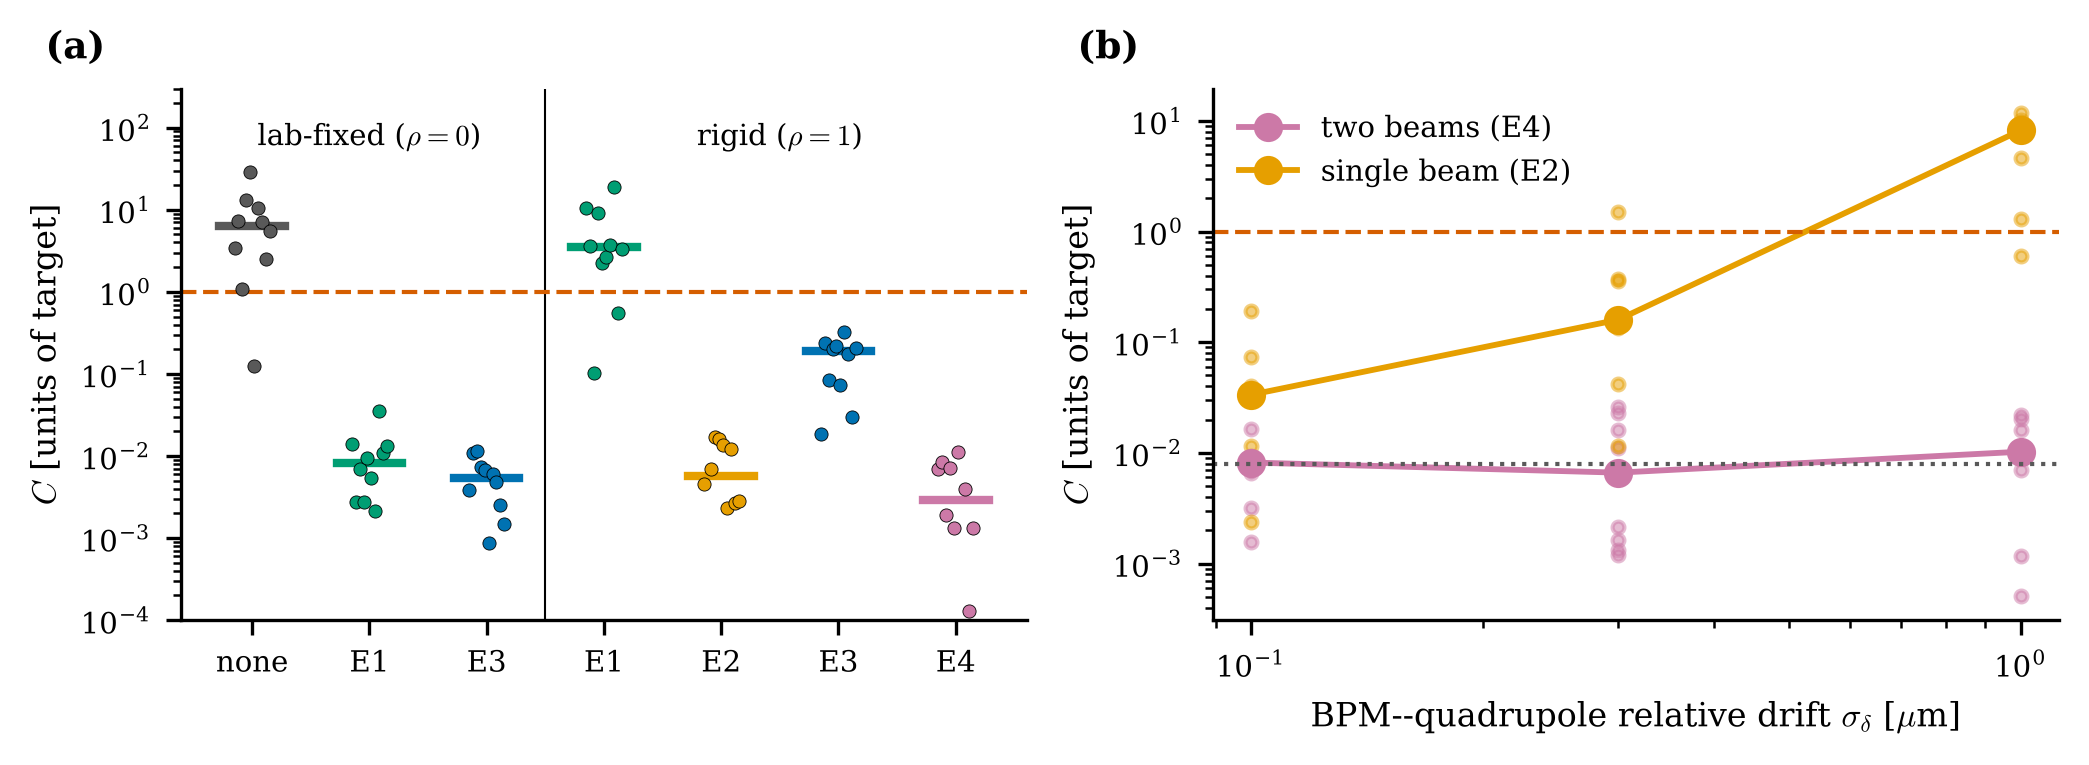
\includegraphics[width=\linewidth]{fig_v2_bpm.png}
\caption{Monitor model. (a) False EDM after correction of a 5~$\mu$m symmetric drift for monitors fixed
($\rho=0$) or rigidly attached ($\rho=1$), for the estimators of Table~\ref{tbl:bpm} (10 patterns; bars =
median). (b) Rigidly attached monitors with relative BPM--quadrupole drift $\sigma_\delta$ (8 patterns).
Dashed: target; dotted: numerical floor.}
\label{fig:bpm}
\end{figure*}

\subsection{Electrostatic deflector errors}
\label{sec:defl}
A relative field error $\varepsilon$ of one deflector deflects the beam horizontally, a roll $\phi$ about
the beam axis adds a vertical field $E_y\approx E_0\phi$. For $\varepsilon=10^{-4}$ and $\phi=0.1$~mrad in
a single deflector the closed-orbit distortion reaches 418 and 525~$\mu$m, confirming the estimate of
$\sim400~\mu$m. Since the electric force does not reverse with the beam direction, these orbits are the same
for both beams (correlation $+0.95$) and fall entirely in the sum channel, where they compete with the
symmetric quadrupole drift.

\paragraph*{Orbit.} A fit containing only quadrupole columns mistakes a deflector drift for a symmetric
misalignment: about 1~$\mu$m per $10^{-7}$ in $\varepsilon$ or per 0.1~$\mu$rad in $\phi$
[Fig.~\ref{fig:deflector}(a)]. Adding the 48 deflector columns per plane keeps the problem full rank (96
unknowns, 96 readings) but raises its condition number from 73 (118) to $5.6\times10^3$ ($7.9\times10^3$)
horizontally (vertically), because a few deflector and quadrupole patterns produce nearly the same orbit
(principal-angle cosines above 0.99 in 4--6 directions; both drive the harmonics near the tune). The
leakage then disappears: the symmetric error stays at 0.036~$\mu$m with an exact model and rises to
0.4~$\mu$m at $\varepsilon=10^{-5}$ with a 0.2\% gradient error; the price is a doubling of the noise
amplification.

\paragraph*{Spin, first order.} A deflector roll gives a vertical electric kick $\theta_E=(2\pi/48)\phi$.
The closed orbit balances it by magnetic kicks in the quadrupoles, $\sum\theta_B=-\sum\theta_E$, and the
magnetic field rotates the spin $G\gamma$ times more than the momentum. The result is a first-order
out-of-plane precession $f=G\gamma\sum\theta_E/T_\text{rev}$, reproduced by the tracking to $10^{-5}$ (for
$3\times10^{-7}$ rms rolls, $1.26\times10^8\times$ target). It has the same sign for both beams and cancels
in $C$ to the numerical precision; in a real ring the cancellation is limited by the CW/CCW asymmetry,
which must be below $\sim10^{-8}$ for rolls of this size. This is a general requirement of the
experiment, addressed in Ref.~\cite{omarov}.

\paragraph*{Spin, second order, and deflector trims.} Field errors and rolls together produce horizontal
and vertical closed orbits whose product generates a geometric phase of its own, $C\approx1$ for
$\varepsilon,\phi\sim3\times10^{-7}$ even with perfectly aligned quadrupoles. Correcting the quadrupoles
alone does not remove it (with a 0.2\% gradient error: $C=0.75$ median, 3 of 8 patterns above target). The
remedy is to trim the deflectors at the source, using the deflector part of the fit: the field error by the
deflector voltage, the roll by a small voltage difference between the upper and lower electrodes. Individual
deflector errors are poorly estimated (25--80\% remains), but the poorly estimated directions are exactly
those with little orbit effect; the deflector-induced orbit is reduced by 97--99\%, and the false EDM falls
to $C=0.010$ (0.016 with a 0.2\% gradient error). Figure~\ref{fig:deflector}(b) scans the amplitude of the
deflector drift: with an exact model the trimmed result stays at the floor up to $10^{-5}$, because the
estimation error is set by the BPM noise only; with a 0.2\% gradient error it grows as the square of the
amplitude and reaches the target at 3--5$\times10^{-6}$. The tolerable deflector drift between trims is
therefore set by the accuracy of the response model. For comparison, present high-voltage supplies quote
$10^{-5}$ ripple~\cite{cpedm_feas} and $10^{-4}$ long-term stability~\cite{fug}; common-mode changes are
absorbed by the frozen-spin feedback, and only independent slow drifts between trim updates matter.

\begin{figure*}[tb]
\centering
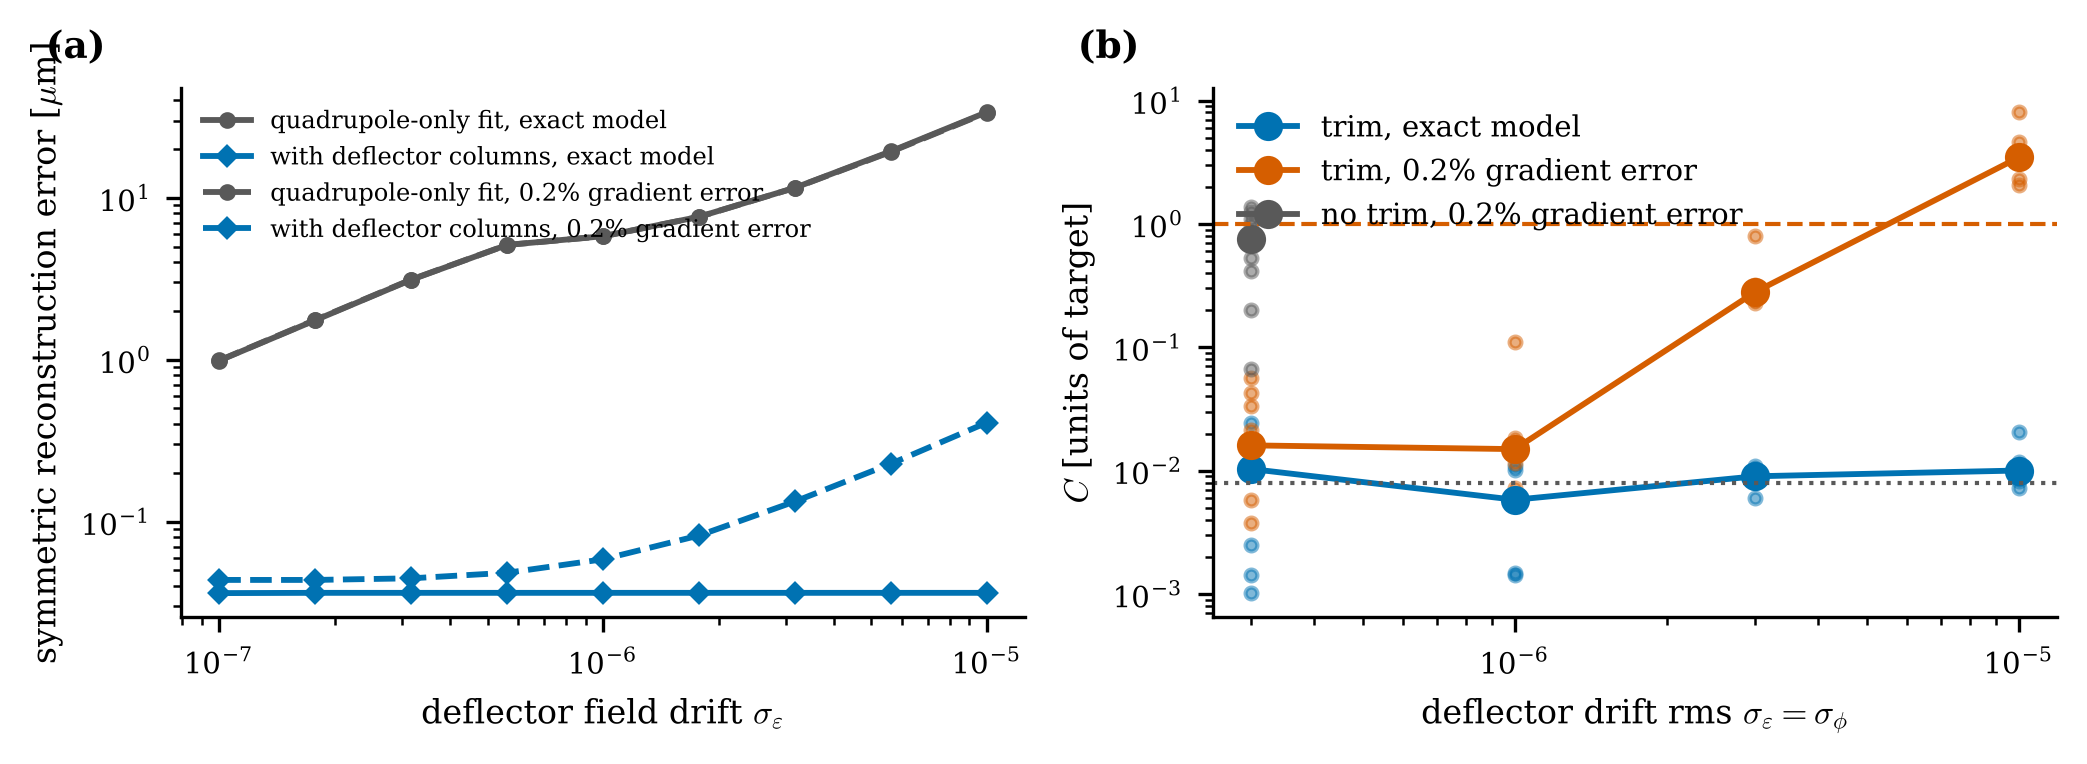
\includegraphics[width=\linewidth]{fig_v2_deflector.png}
\caption{Deflector errors. (a) Error of the reconstructed symmetric quadrupole drift (5~$\mu$m, horizontal
plane, 200 patterns) versus deflector field drift, for a fit with quadrupole columns only and with
deflector columns added. (b) False EDM after quadrupole correction and deflector trim versus the deflector
drift amplitude (4--8 patterns).}
\label{fig:deflector}
\end{figure*}

\subsection{Corrector type}
\label{sec:correctors}
The scheme of Sec.~\ref{sec:croc} needs a corrector that cancels the misalignment where it occurs. A dipole
winding in the quadrupole adds a uniform field $\Delta B$ and shifts the magnetic center by $\Delta B/g$, so
with $\Delta B=g\,\Delta\hat v$ the quadrupole acts as aligned for both beams and for the spin; this is the
correction assumed above (quadrupole movers are equivalent). Correctors at the deflectors cannot do this.
Magnetic correctors there kick the two beams in opposite directions and act only in the difference channel,
whereas a symmetric drift requires a same-sign displacement of both beams; zeroing the BPM readings leaves
the beam off the quadrupole centers. Electrostatic correctors act on both beams alike and can steer them
through the quadrupole centers (within 0.1~$\mu$m), but the electric kicks they need ($5$--$8\times10^{-6}$
in $\varepsilon$ and $\phi$) generate the first-order and second-order deflector effects described above:
$C=7.6$ (zeroing the readings) and $C=1.3$ (steering to the centers), with first-order same-sign signals of
$10^6$--$10^8\times$ target that rely entirely on CW/CCW symmetry. Only quadrupole-mounted correctors keep
$C$ at the floor.

\subsection{Correlated misalignment}
\label{sec:correlated}
Survey errors and ground motion produce misalignments correlated along the ring, with the relative
displacement of two quadrupoles growing as the square root of their distance. We modeled this by a periodic
random walk ($\langle(v_i-v_j)^2\rangle\propto|s_i-s_j|$, the spatial structure of the ATL law
$\langle\Delta Y^2\rangle=ATL$~\cite{shiltsev}), with the trivial rigid translation and tilt removed.
Because neighboring quadrupoles move together, the symmetric component dominates: the symmetric-to-
antisymmetric rms ratio is 2.3 (84\% of the variance) against about one for uncorrelated errors (2000 patterns).
Correlation therefore makes the symmetric component more important, which strengthens the case for a
scheme that reads it. The two-beam correction itself is linear and insensitive to the pattern statistics:
after correction the residual is at the noise level for uncorrelated, random-walk and mixed models alike.
If the ground motion also moves the monitors, the situation is that of Sec.~\ref{sec:bpm} with $\rho\approx1$:
a fixed-monitor estimator then recovers only about 30\% of the symmetric drift, whereas an estimator with
$\rho=1$ recovers it to 0.01~$\mu$m.
\todo{The false-EDM values of the correlated models (old estimator, all $\le0.005$ after correction) are not
quoted; at these small residual orbits the launch bias is negligible (App.~A), but a frozen-spin re-run would
make it explicit.}

%======================================================================
\section{OPERATING SCENARIO}
\label{sec:time}
%======================================================================
To show how the scheme performs in operation we followed the machine for one week in 1~h steps. The
quadrupoles drift according to the ATL law with $A=10^{-5}~\mu$m$^2$/(s\,m), close to the value measured
at LEP~\cite{shiltsev}. After each BBA the residual misalignment is 0.3~$\mu$m rms; the
BPM--quadrupole relative drift $\delta$ grows as $0.2~\mu$m$/\sqrt{\text{day}}$, and BBA is repeated when
its expected value reaches 0.3~$\mu$m (every $\approx54$~h). BPM readings have $10~\mu$m single-turn
resolution averaged over 60~s and a 10~nm floor. We compared rigidly attached monitors with two-beam (E4)
and single-beam (E2) correction, monitors on separate supports that move with the ground but are treated as
fixed (E3), periodic BBA alone, and no correction.

Figure~\ref{fig:time} shows the result. Two-beam monitoring keeps the false EDM at the level set by the
BBA residual throughout the week (median $C=0.05$--$0.09$, largest of 15 values 0.18; $C=0.06$ right after
BBA). Single-beam monitoring and the fixed-monitor model hover around the target (median up to 1.2 and 1.3,
with 3 and 4 of 5 patterns above target at 96~h). Periodic BBA alone rises to $C\approx45$ between
calibrations. The monitor detects a symmetric drift of $3k\sigma_n$, where $k=0.75$ is the noise gain of
the two-beam symmetric estimate and $\sigma_n$ the BPM noise per reading; with a 10~nm floor this is
$\approx0.02~\mu$m.

\begin{figure*}[tb]
\centering
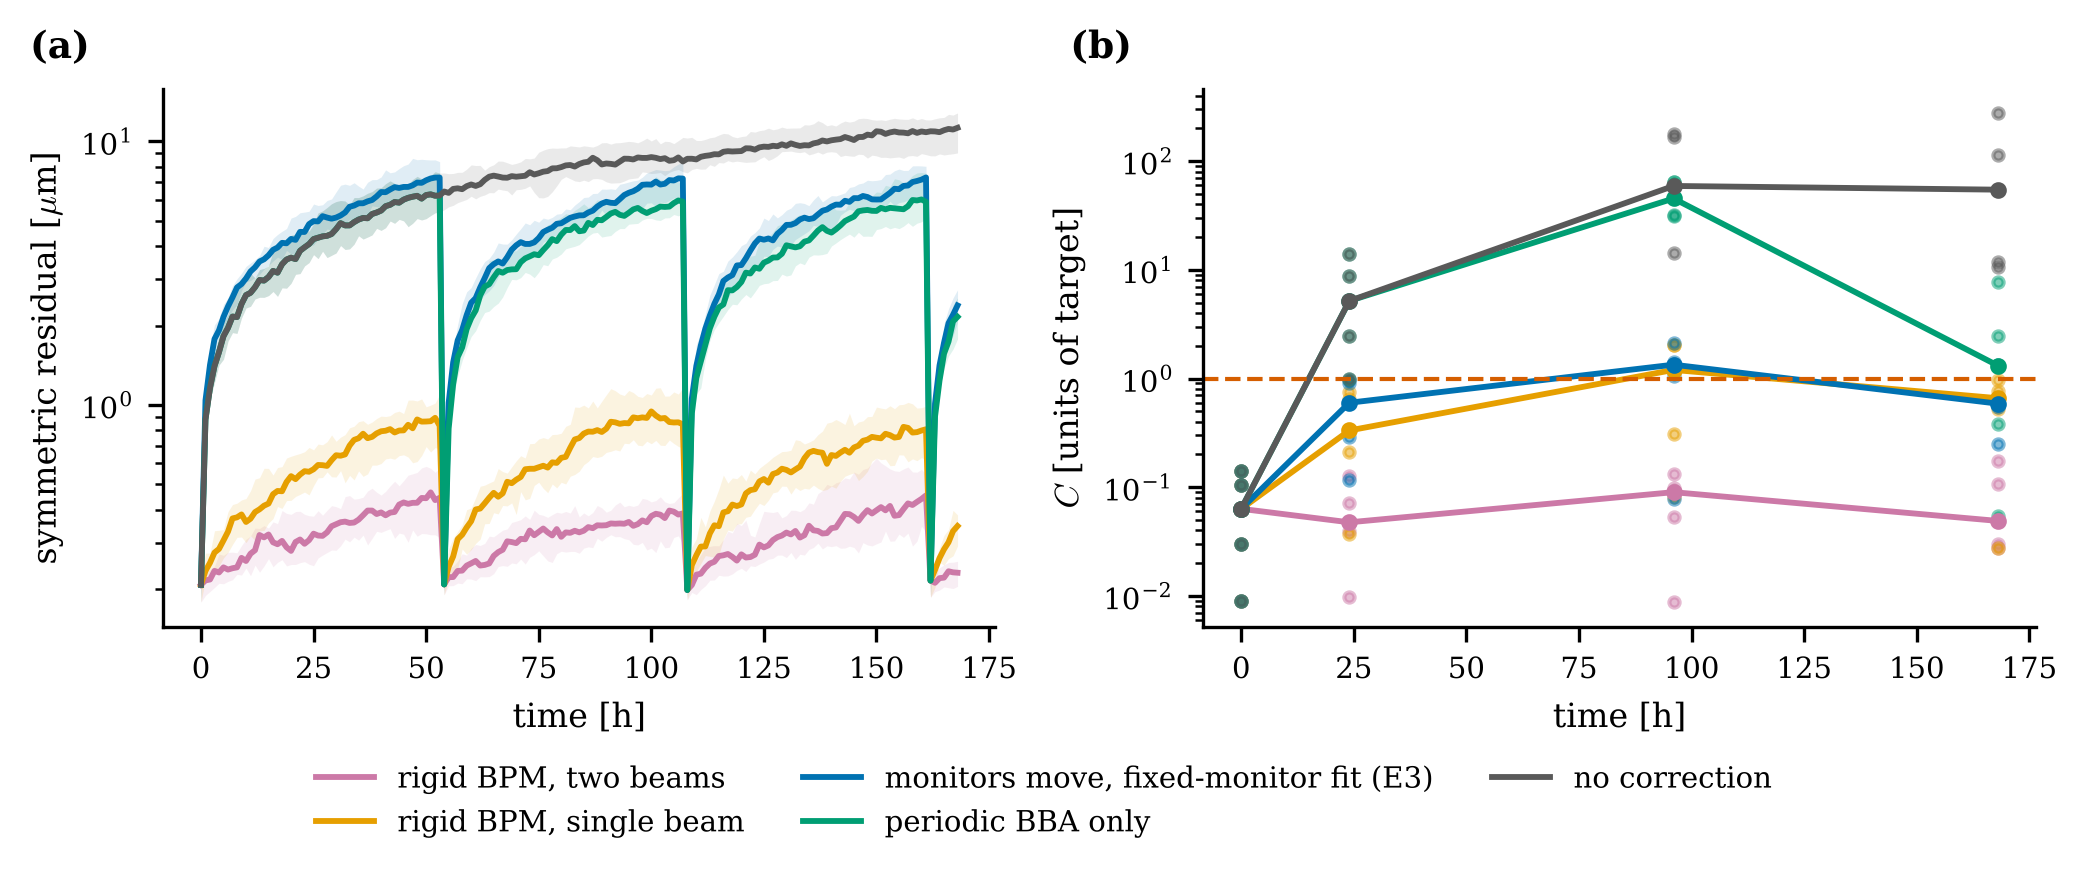
\includegraphics[width=\linewidth]{fig_v2_time.png}
\caption{One-week operating scenario. (a) Residual symmetric misalignment (linear model, 20 patterns,
median and 16--84\% band). (b) False EDM from tracking (5 patterns; lines = median). BBA is repeated at
54, 108 and 162~h.}
\label{fig:time}
\end{figure*}

%======================================================================
\section{CONCLUSIONS}
\label{sec:conclusion}
%======================================================================
The false EDM from quadrupole misalignment is a bilinear functional of the horizontal and vertical
misalignment patterns. Split into symmetric and antisymmetric components, the symmetric component is four
to seven times less visible to the closed orbit at low harmonics---because of the $\beta$ modulation between
QF and QD, not the smooth-focusing suppression---while its weight in the false EDM is reduced by a smaller factor.
Single-beam orbit correction therefore leaves it largely in place unless the truncation is chosen
carefully.

The two counter-rotating beams separate the components: the antisymmetric one in the difference of the two
orbits, the symmetric one in their sum. Because static BPM offsets are degenerate with the symmetric
component in the sum, the scheme is a drift monitor between BBA calibrations, and it does not need the
quadrupole polarity reversal of the reference scheme. Its domain of validity is set by the errors that
share the sum channel:
\begin{itemize}
\item the monitor model must match the mounting; rigidly attached monitors with a model that knows it
make the scheme robust against BPM--quadrupole drifts up to at least 1~$\mu$m and against 10\% errors in
the mounting coefficient;
\item deflector drifts must be included in the fit and trimmed at the source; the tolerable drift between
trims, $\sim3\times10^{-6}$ with a 0.2\% gradient error, scales with the accuracy of the response model;
\item the corrections must be applied by quadrupole-mounted dipole correctors (or movers);
\item first-order effects of deflector rolls cancel only through the CW/CCW symmetry of the ring.
\end{itemize}
Within these conditions, two-beam monitoring keeps the false EDM well below target between BBA
calibrations over a week of simulated operation.

Finally, the false EDM in a misaligned lattice must be evaluated at the frozen-spin energy, which differs
from the design magic energy by an amount proportional to the misalignment; a fixed-momentum evaluation
depends on the launch point and can differ by orders of magnitude.

\begin{acknowledgments}
This work was supported by the Scientific and Technological Research Council of T\"urkiye (T\"UB\.ITAK)
under the 1001 Program (Project No.~123F256).
Generative AI tools (Claude, Anthropic) were used to assist in software development, simulation
campaigns, figure generation and drafting. All scientific methodology, validation, interpretation and
conclusions were performed and verified by the authors.
\todo{Authors to confirm the AI-use statement.}
\end{acknowledgments}

\appendix

\section{Frozen-spin evaluation and launch-point dependence}
\label{app:launch}
For the misalignment patterns used here the false EDM evaluated at fixed momentum
($|p|=p_\text{magic}$ at the launch point) and at the frozen-spin energy differ by an amount proportional to
the closed-orbit amplitude at launch. For the patterns of Fig.~\ref{fig:suppression}, the difference is
$\le0.02\times$ target after two-beam correction (rms orbit product $\approx0.01~\mu$m$^2$), $\le0.2$ for
the corrected beam after single-beam correction ($\approx1~\mu$m$^2$), and 1--3000 for the uncorrected
beam and uncorrected machine ($10^2$--$10^4~\mu$m$^2$). Because the error differs between the two beam
directions, it does not cancel in $C$. The frozen-spin result does not depend on the starting rule of the
interpolation: starting from the fixed-momentum rule, the frozen-spin energy found at four launch points
agrees to four digits with the momentum profile of the frozen-spin orbit, and a measurement taken there
gives $82.04$ and $81.87$ against $82.04$ and $81.90$ from the default rule. If the second interpolation
point is far from $\omega_h=0$ ($|\omega_1|>10^{-3}$~rad/s), a third measurement at the interpolated energy
is taken.

\section{Optics breathing}
\label{app:breathing}
Changing the gradient of one quadrupole slightly changes the betatron functions of the whole ring and
therefore every response-matrix element [Eq.~\eqref{Eq:response_matrix}]. When all quadrupoles are
modulated at different frequencies, these changes dominate the reconstruction (Fig.~\ref{fig:breathing}).

\begin{figure}
\centering
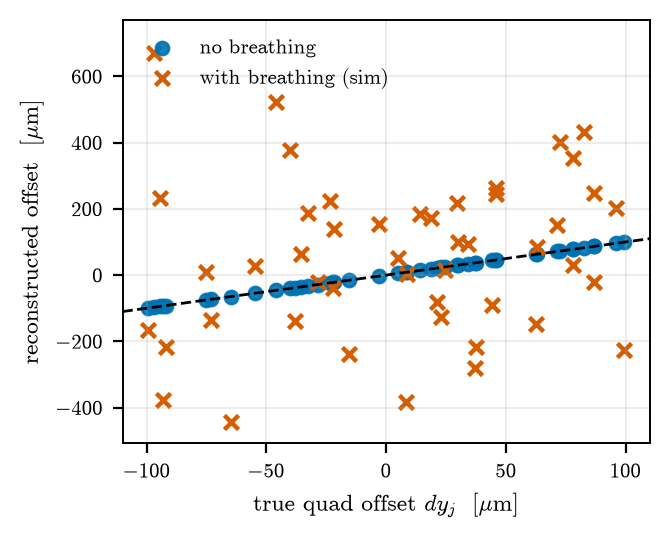
\includegraphics[width=1\linewidth]{fig_orbit_breathing.png}
\caption{Reconstruction of misalignments when the quadrupoles are modulated. If the breathing effect is
artificially removed, the reconstruction works; with it, the signal is buried.}
\label{fig:breathing}
\end{figure}

\section{Inversion of the orbit difference}
\label{app:orb_diff_inv}
The orbit difference between two gradient settings cancels static offsets. If the gradient changes by
$\epsilon_g$, the difference matrix scales as $\Delta R\approx\epsilon_g\,\partial R/\partial g$, so that
$\|\Delta R^{-1}\|\approx\|R^{-1}\|/\epsilon_g$; its condition number is $3.7\times10^4$ for this lattice.
Because the smallest singular values belong to symmetric directions, the inversion fails selectively for
the symmetric component (Fig.~\ref{fig:orbit_lock}); regularization removes the same directions.

\begin{figure}
\centering
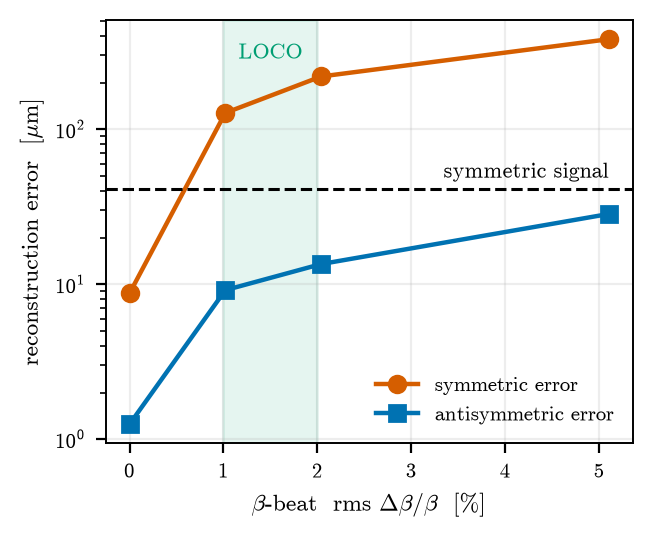
\includegraphics[width=1\linewidth]{fig_orbit_lockin.png}
\caption{Reconstruction error of the orbit-difference approach versus $\beta$-beat. The error of the
symmetric component becomes about 15 times larger than that of the antisymmetric one.}
\label{fig:orbit_lock}
\end{figure}

\section{Two-dimensional illustration of the counter-rotating sum}
\label{app:sum}
Represent the misalignment in one plane by $v=(a,s)^{\top}$, one antisymmetric and one symmetric
coordinate. The antisymmetric one drives a large orbit and the symmetric one a small orbit, so
$R_\text{CW}=\mathrm{diag}(G,g)$ with $G\gg g$. Beam reversal flips the antisymmetric orbit but, up to a
phase shift, not the symmetric one: $R_\text{CCW}=\mathrm{diag}(-G,g)$. Every reading carries the static
offset $b=(b_a,b_s)^{\top}$ of its monitor, common to both beams. Then
\begin{equation}
\begin{split}
y_\text{CW}-y_\text{CCW} &= (2Ga,\ 0)^{\top},\\
y_\text{CW}+y_\text{CCW} &= (2b_a,\ 2gs+2b_s)^{\top}.
\end{split}
\label{eq:sumdiff}
\end{equation}
The difference gives $a$ free of offsets and well conditioned; the sum gives $s$ only together with the
offset $b_s$, through the small gain $g$. A static symmetric misalignment and a static offset are
degenerate in a single measurement, but the offset cancels in the change of the sum,
$\Delta s=\Delta(y_\text{CW}+y_\text{CCW})/2g$, which is why the scheme is a drift monitor. In the ring,
$v$ has 48 entries per plane and each beam gives 48 readings, and the components are obtained by the
least-squares solution of Eq.~\eqref{eq:twobeamfit}. In a real ring the parity is approximate---the beams
cross each cell in opposite order---so the antisymmetric orbit leaves a small residual in the sum
[Fig.~\ref{fig:orbit_cw_ccw}(a)].

\begin{thebibliography}{99}
\bibitem{srEDM}
V.~Anastassopoulos \emph{et al.},
``A storage ring experiment to detect a proton electric dipole moment,''
Rev.\ Sci.\ Instrum.\ \textbf{87}, 115116 (2016).

\bibitem{omarov}
Z.~Omarov, H.~Davoudiasl, S.~Hac{\i}\"omero\u{g}lu, V.~Lebedev, W.~M.~Morse, Y.~K.~Semertzidis,
A.~J.~Silenko, E.~J.~Stephenson, and R.~Suleiman,
``Comprehensive symmetric-hybrid ring design for a proton EDM experiment at below
$10^{-29}\,e\!\cdot\!$cm,''
Phys.\ Rev.\ D \textbf{105}, 032001 (2022).

\bibitem{polarimeter}
F.~M\"uller \emph{et al.} (JEDI Collaboration),
``A new beam polarimeter at COSY to search for electric dipole moments of charged particles,''
J.\ Instrum.\ \textbf{15}, P12005 (2020).

\bibitem{berry1984}
M.~V.~Berry, ``Quantal phase factors accompanying adiabatic changes,''
Proc.\ R.\ Soc.\ Lond.\ A \textbf{392}, 45 (1984).

\bibitem{aharonov1987}
Y.~Aharonov and J.~Anandan, ``Phase change during a cyclic quantum evolution,''
Phys.\ Rev.\ Lett.\ \textbf{58}, 1593 (1987).

\bibitem{farley2004}
F.~J.~M.~Farley \emph{et al.},
``New method of measuring electric dipole moments in storage rings,''
Phys.\ Rev.\ Lett.\ \textbf{93}, 052001 (2004).

\bibitem{haciomeroglu2019}
S.~Hac{\i}\"omero\u{g}lu, Y.~F.~Orlov, and Y.~K.~Semertzidis,
``Magnetic field effects on the proton EDM in a continuous all-electric storage ring,''
Nucl.\ Instrum.\ Methods A \textbf{921}, 12 (2019).

\bibitem{marti}
Z.~Mart\'{\i}, G.~Benedetti, U.~Iriso, and A.~Franchi,
``Fast beam-based alignment using ac excitations,''
Phys.\ Rev.\ Accel.\ Beams \textbf{23}, 012802 (2020).

\bibitem{huang}
X.~Huang, ``Simultaneous beam based alignment measurement for multiple magnets,'' arXiv:2203.14869.

\bibitem{chung1993}
Y.~Chung, G.~Decker, and K.~Evans,
``Closed orbit correction using singular value decomposition of the response matrix,''
in \emph{Proceedings of PAC 1993}, p.~2263.

\bibitem{ziemann}
V.~Ziemann and M.~Ziemann,
``Noninvasively improving the orbit response matrix while continuously correcting the orbit,''
arXiv:2104.05300.

\bibitem{mirza}
S.~H.~Mirza, R.~Singh, P.~Forck, and H.~Klingbeil,
``Closed orbit correction at synchrotrons for symmetric and near-symmetric lattices,''
Phys.\ Rev.\ Accel.\ Beams \textbf{22}, 072804 (2019).

\bibitem{wegscheider}
S.~Wegscheider, J.~Vilsmeier, \emph{et al.},
``Inverse modeling of circular lattices via orbit response in the presence of degeneracy,''
Phys.\ Rev.\ Accel.\ Beams \textbf{26}, 032803 (2023).

\bibitem{hairer}
E.~Hairer, C.~Lubich, and G.~Wanner,
\emph{Geometric Numerical Integration}, 2nd ed.\ (Springer, Berlin, 2006).

\bibitem{bmt1959}
V.~Bargmann, L.~Michel, and V.~L.~Telegdi,
``Precession of the polarization of particles moving in a homogeneous electromagnetic field,''
Phys.\ Rev.\ Lett.\ \textbf{2}, 435 (1959).

\bibitem{jedi_phaselock}
N.~Hempelmann \emph{et al.} (JEDI Collaboration),
``Phase locking the spin precession in a storage ring,''
Phys.\ Rev.\ Lett.\ \textbf{119}, 014801 (2017).

\bibitem{rossbach}
J.~Rossbach,
``Closed-orbit distortions of periodic FODO lattices due to plane ground waves,''
Part.\ Accel.\ \textbf{23}, 121 (1989).

\bibitem{shiltsev}
V.~Shiltsev, ``Observations of random walk of the ground in space and time,''
Phys.\ Rev.\ Lett.\ \textbf{104}, 238501 (2010).

\bibitem{ttf2}
TTF2 BPM--quadrupole calibration on a stretched-wire bench, in \emph{Proceedings of LINAC 2004}, TUP69.
\todo{Complete author list and title.}

\bibitem{pacman}
CLIC/PACMAN BPM--quadrupole pre-alignment, PhD thesis, Univ.\ of Pisa (2016),
\url{https://etd.adm.unipi.it/t/etd-12172016-033103/}.
\todo{Complete author and title.}

\bibitem{sls2}
``Development of the SLS 2.0 BPM system,'' in \emph{Proceedings of IBIC 2023}, MO3C03.
\todo{Complete author list.}

\bibitem{aps_mba}
R.~Lill, N.~Sereno, and B.~Yang, ``BPM stability studies for the APS MBA upgrade,''
\url{https://www.osti.gov/servlets/purl/1393935}.

\bibitem{cpedm_feas}
F.~Abusaif \emph{et al.} (CPEDM Collaboration),
``Storage ring to search for electric dipole moments of charged particles: Feasibility study,''
CERN Yellow Reports: Monographs, CERN-2021-003; arXiv:1912.07881.

\bibitem{fug}
P.~Schmidt-Wellenburg and T.~Schmidt,
``The FuG HCB 200~kV bipolar high-voltage power supply for the storage chamber in a nEDM experiment,''
presentation (2020).
\todo{Replace with a citable source if available.}
\end{thebibliography}

\end{document}
